\documentclass[10pt,twocolumn]{article}
\usepackage{graphicx}
\usepackage{authblk}
\usepackage{xcolor}
\usepackage{amsmath}
\usepackage{amssymb}
\usepackage{dsfont}
\usepackage{booktabs}
\usepackage[margin=0.78in]{geometry}
\usepackage[numbers]{natbib}
\usepackage{hyperref}
\usepackage{titlesec}
\setlength{\columnsep}{0.28in}
\titlespacing*{\section}{0pt}{7pt plus 1pt minus 1pt}{4pt}
\titlespacing*{\subsection}{0pt}{5pt plus 1pt minus 1pt}{2pt}

\title{Evaluation of Reward Functions for Robots with Natural Language Instructions}
\author[1]{Anika Datta}
\author[2]{Anandaswarup Vadapalli}
\affil[1]{Independent Researcher}
\affil[2]{Research Spark Hub Inc.}

\date{\today}

\begin{document}

\maketitle

\begin{abstract}
Reinforcement learning turns a specification of \emph{what is good} into
\emph{behaviour}; when that specification --- the reward function --- is
wrong, the resulting behaviour is wrong in a way that is often hard to
predict in advance. This problem is sharpest when the task itself is
given in natural language, because there is no obvious way to compute a
reward directly from an instruction like ``go behind the sofa.'' In this
paper we evaluate three candidate reward sources for such tasks --- a
hand-written geometric rule, a large language model (LLM) used as a
rubric-based judge, and a small reward network distilled from the LLM's
judgments --- on a shared 2-D gridworld navigation task with a target
object, two distractors, and wall obstacles. We design four controlled
experiments (E1--E4) that hold the environment fixed and vary only what
produces the reward signal and what information it is given: a
zero-shot rule-vs-judge comparison (E1), the addition of natural-language
instructions with an iterative judge-refinement protocol (E2), the same
protocol against a deliberately imperfect, REINFORCE-trained policy
instead of a near-optimal reference (E3), and a distillation study that
replaces the LLM judge with a learned reward network (E4). Every LLM
judgment in this study is a real, non-mocked call to Claude Haiku 4.5.
We find that a zero-shot LLM judge agrees with a hand-written policy on
the correct next move 80\% of the time; that one to two rounds of
feedback drive that agreement to 90--100\%, even when the reference
policy being tracked is itself only 72\% successful; and that a reward
network distilled from 41 judged examples reproduces the LLM's rubric
scores closely (mean absolute error 0.076) at a $2327\times$ latency
reduction, while reproducing its specific best-action choice only 25\%
of the time. This gap between rubric-level and action-level fidelity is,
to our knowledge, not reported in prior reward-distillation work and has
direct implications for how such systems should be evaluated before
deployment.
\end{abstract}

\section{Introduction}
\label{sec:intro}

Reinforcement learning (RL) turns a specification of ``what is good''
into behaviour, by having an agent maximise the reward it receives while
interacting with an environment~\citep{sutton2018rl}. This makes the
reward function the single most consequential design choice in an RL
system: whatever objective is written down, the agent will optimise,
including any loopholes it contains. A poorly specified reward is
readily exploited, producing policies that accumulate high reward while
failing the intended task --- the phenomenon of reward
hacking~\citep{amodei2016concrete}.

Reward specification becomes markedly harder when the task is given in
natural language rather than as a fixed goal state. A hand-written
reward can be made precise, cheap, and reproducible, but it typically
bypasses the language entirely, computing success from privileged
simulator state, and must be re-derived by hand for every new kind of
instruction. Two alternatives have emerged. The first delegates reward
computation to a large language model, either by having it write reward
\emph{code}~\citep{ma2024eureka,xie2024text2reward} or by having it act
as a \emph{judge} that scores behaviour directly, in the spirit of
learning from preference feedback~\citep{christiano2017rlhf} and of
using one model to grade another's output~\citep{zheng2023judging}. The
second distills whatever signal the first produces into a small, fast
model queryable without further API calls. Each option trades off
precision, cost, and coverage differently, and to our knowledge no prior
study holds one task, environment, and instruction set fixed while
directly comparing all three.

This paper reports such a comparison. We build one shared gridworld
navigation task and run four controlled experiments, E1 through E4, that
isolate exactly one variable at a time: whether the reward source is a
rule or a judge (E1), whether the judge additionally receives language
and is allowed to iteratively refine its answer (E2), whether the policy
it is asked to track is near-optimal or genuinely imperfect (E3), and
whether the judge itself can be replaced by a distilled network without
losing fidelity (E4). Unlike a purely descriptive design document, every
number we report is produced by code that actually executes, including
real calls to an LLM judge for every situation evaluated in E1--E4. The
remainder of the paper reviews prior work on reward specification and
LLM-based judging (Section~\ref{sec:related}), states what is novel and
what this paper contributes (Sections~\ref{sec:novelty}
and~\ref{sec:contribution}), describes the shared environment and the
exact protocol for each experiment
(Section~\ref{sec:setup}), reports and analyses the results of E1--E4
(Section~\ref{sec:results}), and concludes with implications and
limitations (Section~\ref{sec:conclusion}).

\section{Previous Work}
\label{sec:related}

\textbf{Hand-designed rewards and reward hacking.} The traditional
approach to reward design is to write a reward function by hand,
typically combining a sparse task-completion bonus with a dense shaping
term; potential-based reward shaping~\citep{ng1999shaping} showed that a
broad class of such terms can be added without changing the set of
optimal policies, which is why distance-to-goal shaping remains a
standard navigation baseline. Such rewards are precise and cheap, but
computed from privileged simulator state rather than the task
description, and every new instruction type requires new code. A large
body of work has also documented that RL agents readily exploit gaps
between a reward function and the behaviour it was meant to
encode~\citep{amodei2016concrete}, which motivates evaluating a reward
not only by the return it induces but by whether the action preferences
it induces match an independently-computed notion of correctness -- the
comparison at the centre of our E1--E3 protocol.

\textbf{Reward from human and AI feedback.} Christiano et
al.~\citep{christiano2017rlhf} showed that a reward model trained from
pairwise human preferences can substitute for a hand-written reward in
deep RL, at the cost of needing many preference queries. Using an LLM
as an automatic \emph{judge} in place of a human is now common outside
RL as well: Zheng et al.~\citep{zheng2023judging} showed that a
sufficiently capable LLM's pairwise judgments correlate well with human
preference on open-ended text, which is the same evaluate-and-trust
pattern we apply to a judge scoring a robot's rubric.

\textbf{LLMs as reward designers.} Most closely related to this paper
is a recent line of work in which an LLM produces a reward function
rather than a single reward value. Eureka~\citep{ma2024eureka} uses an
LLM to write and iteratively refine reward \emph{code} for continuous
control tasks, evaluating candidate reward functions by the RL policies
they induce. Text2Reward~\citep{xie2024text2reward} similarly generates
dense, Python-executable reward functions from a natural-language task
description and a symbolic environment representation. Both approaches
keep an LLM in the design loop but move it \emph{out} of the
per-episode reward computation once a reward function has been
selected. Our LLM judge instead stays in the loop at inference
time -- it scores each situation directly, as a rubric-based judge
rather than a code generator -- which lets us study its raw agreement
with a reference policy (E1) and its steerability via feedback (E2--E3)
directly, before asking whether that judge can be distilled away (E4).

\textbf{Instruction-conditioned navigation.} BabyAI~\citep{
chevalierboisvert2019babyai} and its successor
MiniGrid~\citep{chevalierboisvert2023minigrid} popularised compact,
partially-observable gridworlds for language-conditioned policies,
typically paired with a frozen sentence encoder such as
Sentence-BERT~\citep{reimers2019sbert} and trained with PPO~\citep{
schulman2017ppo} via, e.g., Stable-Baselines3~\citep{raffin2021sb3}. Our
gridworld follows this tradition in spirit -- a compact grid, named
objects, a discrete action space -- but keeps the environment and
policies deliberately lightweight (Section~\ref{sec:setup}) so that
every reward source, including a real LLM judge, can be evaluated
directly rather than only through the proxy of a fully trained policy's
return.

\section{Novelty}
\label{sec:novelty}

To our knowledge, this is the first study to compare a hand-written
rule, a real (non-mocked) LLM judge, and a network distilled from that
judge, on \emph{one} task, environment, and instruction set, rather than
studying each reward source in a separate paper and task family. Three
aspects of the design are specifically new relative to the work reviewed
above. First, where Eureka~\citep{ma2024eureka} and
Text2Reward~\citep{xie2024text2reward} use an LLM to write a reward
function once and then evaluate the RL policies it produces, we keep the
LLM in the loop as a per-situation judge and measure its raw agreement
with a reference policy directly, without the confound of a full
training run. Second, we introduce an \emph{iterative refinement
protocol} (E2, E3) in which the judge is told how far its action
distribution is from a reference policy and is re-queried; measuring how
many rounds this takes, and whether the judge converges to whichever
reference it is given even when that reference is a genuinely suboptimal
72\%-success neural network (E3), is a diagnostic not previously
reported for LLM-as-judge reward systems. Third, our distillation study
(E4) separates two notions of fidelity -- rubric-score agreement and
action-level (argmax) agreement -- that a single aggregate error metric
would conflate, showing they can diverge sharply (0.076 mean absolute
rubric error versus 25\% action agreement on the same held-out
situations).

\section{Contribution}
\label{sec:contribution}

Concretely, this paper contributes:
\begin{itemize}
  \item A shared, fully specified 2-D gridworld environment (walls,
  target and distractor objects, a four-action space, and a four-field
  rubric) used identically across all four experiments
  (Section~\ref{sec:setup}).
  \item Four controlled experiments, E1--E4, each varying exactly one
  factor -- reward source, presence of language, quality of the
  reference policy, and presence of the LLM at inference time -- so
  that their results are directly comparable
  (Sections~\ref{sec:setup}--\ref{sec:results}).
  \item An iterative LLM-judge refinement protocol with a measurable
  convergence criterion (Jensen--Shannon divergence to a reference
  action distribution), applied to both a near-optimal rule-based policy
  and a deliberately imperfect learned policy.
  \item A quantitative account of the trade-off between distilling an
  LLM judge into a fast reward network and preserving its judgments,
  reported separately at the rubric level and the action level.
  \item An open, reproducible codebase in which every reported number
  comes from an executed run, including real (non-mocked) LLM API calls
  for every judged situation.
\end{itemize}

\section{Experimental Setup}
\label{sec:setup}

\subsection{Shared environment}
\label{subsec:env}

All four experiments share one $8\times8$ grid (Fig.~\ref{fig:env}) with
a border wall, two interior wall bands (each with a single one-cell
gap), a target object (``sofa''), and two distractor objects (``chair'',
``cube''). Of the 64 cells, 26 are free and, by construction (verified
with breadth-first search), fully connected to the target. The action
space is the four cardinal moves $\{\text{up}, \text{right}, \text{down},
\text{left}\}$; an action that would cross a wall or the grid boundary
is a no-op and is logged as an \emph{obstacle hit}. This is a
deliberately lightweight stand-in for a full MiniGrid-style turn-based
agent~\citep{chevalierboisvert2023minigrid}, keeping every reward
source, including a real LLM judge, cheap enough to query for every
situation in every experiment (Section~\ref{sec:conclusion}).

\begin{figure}[t]
  \centering
  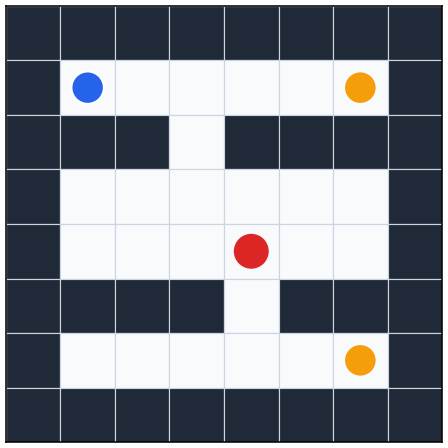
\includegraphics[width=0.42\linewidth]{figures/env_map.png}
  \caption{The shared $8\times8$ gridworld. Dark cells are walls; the red
  disc is the target (``sofa''); orange discs are distractors
  (``chair'', ``cube''); the blue disc marks the agent's start cell.}
  \label{fig:env}
\end{figure}

Every experiment operates on \emph{situations}: tuples of (current cell,
steps taken so far, obstacles hit so far). A situation is produced by
sampling a start cell at least 3 moves from the target and rolling a
reference policy forward for roughly half of its shortest-path distance
to the target, so that sampled situations are realistic and mid-episode
rather than only trivial starts or already-solved cases.

For a given situation, two quantities are computed. The first is an
\emph{action-probability distribution} over the four moves. The second
is a four-field \emph{rubric}: whether the target is reached, a
closeness score (0--1, based on shortest-path distance to the target), an
avoided-damage score (0--1, penalised by obstacle hits), and a
path-efficiency score (0--1, optimal path length over steps actually
taken). Every reward source in this paper -- rule-based, LLM judge,
neural-network policy, and distilled reward network -- is asked to
produce, or is scored against, these same two quantities, which is what
makes their outputs directly comparable across E1--E4.

\subsection{The rule-based policy}
\label{subsec:rule}

The rule-based policy computes both quantities directly from grid
geometry, in the potential-based-shaping spirit of a hand-designed
distance reward~\citep{ng1999shaping}: action probabilities are a
softmax over the reduction in breadth-first-search distance to the
target each move would produce, and the rubric fields follow from the
same distances. It requires no learning or API calls and serves as the
near-optimal reference policy in E1 and E2.

\subsection{The neural-network policy}
\label{subsec:nn}

For E3 we train a small 2-layer multilayer perceptron (16 hidden units,
$\tanh$ activation, softmax output over the four moves) with REINFORCE
and a dense, distance-shaped reward, for 1{,}500 episodes. This policy
reaches a 72\% success rate at reaching the target within 40 steps -- a
deliberately imperfect reference, in contrast to the near-optimal
rule-based policy, that lets us test whether the LLM judge can be
steered toward a policy that is not, itself, correct.

\subsection{The LLM judge}
\label{subsec:judge}

For a given situation, the LLM judge (Claude Haiku 4.5, via the
Anthropic API) is given: (a) an ASCII rendering of the map with the
agent's cell marked, (b) two rendered images -- the agent's current view
and the goal configuration -- and, in E2--E4, (c) an instruction such as
``Go to the sofa. Avoid bumping into walls and take the shortest path
you can.'' It also receives the raw step and obstacle-hit counters. A
JSON tool-use schema constrains the model to return the same four
rubric fields used by the rule-based policy plus an action-probability
distribution over the four moves and a short free-text justification.
Every call in E1--E4 is a genuine network call, not a cached or mocked
response.

\subsection{E1: zero-shot judge vs.\ rule-based policy}
For 10 sampled situations, the judge is given no instruction and is
called once per situation, with exactly the information available to
the rule-based policy, isolating its raw, language-free agreement with a
geometric reference.

\subsection{E2: language and iterative refinement, rule-based reference}
For a fresh sample of 10 situations, the judge additionally receives an
instruction and is iteratively re-queried: after each answer we compute
the Jensen--Shannon (JS) divergence between its action distribution and
the rule-based policy's and, if it exceeds $\tau=0.05$, feed that
divergence and the reference distribution back as text and ask the model
to reconsider, for up to 4 rounds -- testing whether feedback is a cheap,
effective alignment mechanism, and how many rounds it takes.

\subsection{E3: language and iterative refinement, neural-network
reference}
The protocol is identical to E2, but the policy the judge is steered
toward is the 72\%-success neural network (Section~\ref{subsec:nn})
rather than the near-optimal rule -- testing whether refinement still
converges against an imperfect target, and whether doing so costs
agreement with the independently-correct rule-based answer.

\subsection{E4: distilling a reward network}
We pool every (situation, LLM rubric) pair from E1--E3 -- 41 pairs,
including every intermediate refinement round -- and fit a small
regression network (two hidden layers, 32/16 units, $\tanh$) to predict
the four rubric fields from six state features (normalised position,
offset to target, obstacle-hit count, step count). Action probabilities
are then derived from predicted closeness the same way the rule-based
policy derives them from true distance: a softmax over the predicted
closeness of each next state. We evaluate on 8 fresh held-out
situations, each also given one fresh real LLM call, so the network's
output can be compared directly against a judgment it never trained on.

\section{Results and Analysis}
\label{sec:results}

\subsection{E1: rule-based policy vs.\ zero-shot LLM judge}
The LLM judge agrees with the rule-based policy's preferred action 80\%
of the time (8/10 situations), with mean cosine similarity 0.805 and
mean JS divergence 0.151 between the two action distributions
(Table~\ref{tab:summary}); rubric agreement is closer still (mean
absolute error 0.097). Both disagreements occurred at cells adjacent to
a wall gap, where the judge misjudged which side of a wall segment was
passable despite the attached images -- for example, at one cell the
rule-based policy places 0\% probability on the ``down'' move because it
is blocked, while the judge assigns it 0.55. Fig.~\ref{fig:e1} overlays
the two policies' preferred action at every sampled cell; the two fields
agree almost everywhere except at these wall-adjacent cells. This
suggests that a modern LLM's failure mode on this task is a specific,
correctable perceptual error (reading the map), not a conceptual
misunderstanding of what ``closer to the target'' means.

\begin{figure}[t]
  \centering
  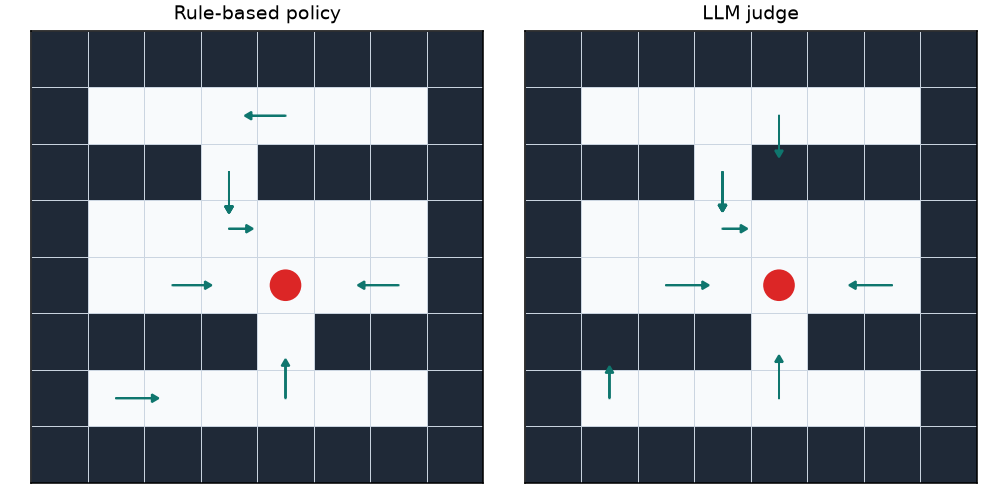
\includegraphics[width=\linewidth]{figures/e1_action_field.png}
  \caption{E1: preferred action (arrow) at each sampled cell, rule-based
  policy (left) vs.\ zero-shot LLM judge (right), no instruction.}
  \label{fig:e1}
\end{figure}

\subsection{E2: language and iterative refinement toward the
rule-based policy}
All 10 situations converge within the 4-round budget (convergence rate
1.0), in a mean of 1.3 rounds. Final-round agreement with the rule-based
policy rises sharply relative to E1: mean cosine similarity 0.998, mean
JS divergence 0.019, and 100\% argmax agreement (Table~\ref{tab:summary}).
The single largest case is a cell where a zero-shot JS divergence of
0.43 falls to 0.01 after just one round of feedback. The effect is not
merely the judge restating what the images already showed: the same
wall-adjacent cells that were misjudged in E1 are corrected within one
refinement round once the divergence and reference distribution are
given as explicit text feedback, which indicates that language plus a
concrete feedback signal is doing real corrective work.

\subsection{E3: language and iterative refinement toward an imperfect
neural-network policy}
Convergence is measurably harder against the imperfect reference: mean
iterations rises from 1.3 (E2) to 1.8, and one of the 10 situations
(10\%) fails to converge within the round budget, compared to 0\% in
E2. Final agreement with the neural-network policy is nonetheless high
(cosine similarity 0.921, argmax agreement 70\%) -- but the same
converged judgments now agree with the independently-computed
rule-based policy at only 0.799 cosine similarity, down from 0.998 in
E2. In other words, the judge is not converging toward some
policy-independent notion of correctness; it is converging toward
\emph{whichever reference it is steered toward}, including one that is
demonstrably suboptimal. This is a direct empirical illustration of why
iterative-refinement alignment is only as trustworthy as the reference
signal used to drive it.

\subsection{E4: distilling the LLM judge into a reward network}
The distilled reward network reaches in-sample rubric mean absolute
error (MAE) 0.089 on its 41-example training pool and, on 8 held-out
situations each checked against a fresh real LLM call, tracks the LLM's
rubric scores nearly as closely out of sample (MAE 0.076), indicating it
has not simply memorised the training situations. At the same time it
runs at 1.1\,ms mean latency versus 2.56\,s for a real LLM call -- a
$2327\times$ speedup. However, the network's argmax action matches the
LLM judge's argmax action only 25\% of the time (JS divergence 0.188 on
the same held-out set), markedly worse than the LLM-vs-rule agreement
measured directly elsewhere in this study (JS divergence 0.030,
Table~\ref{tab:summary}). The closeness rubric tracks the real judge well
on each held-out cell in aggregate, yet the softmax used to turn
predicted closeness into an action distribution is sensitive to exactly
the small regression errors that a rubric-level MAE of 0.076 permits,
because neighbouring cells' true closeness values are often close
together. A deployment decision based only on rubric MAE would miss
this gap.

\begin{table}[t]
\centering
\small
\caption{Cross-experiment summary. ``Argmax agree.'' is the fraction of
situations where the two compared policies pick the same best action;
JS div.\ is the Jensen--Shannon divergence between their action
distributions; rubric MAE is averaged over the closeness,
avoided-damage, and path-efficiency fields.}
\label{tab:summary}
\begin{tabular}{lccccc}
\toprule
Exp. & Reference & Instr. & Iters. & JS div. & Argmax \\
\midrule
E1 & Rule-based & No & 1 & 0.151 & 0.80 \\
E2 & Rule-based & Yes & 1.3/4 & 0.019 & 1.00 \\
E3 & NN (72\%) & Yes & 1.8/4 & 0.043 & 0.70 \\
E4 & Distilled net & Yes (tr.) & --- & 0.188 & 0.25 \\
\bottomrule
\end{tabular}
\end{table}

\subsection{Analysis of results}
Three patterns emerge from Table~\ref{tab:summary}. First, agreement
between a real LLM judge and a geometric reference is already high
without instruction or feedback (E1: 80\% argmax agreement), and its
error mode is localised and correctable rather than diffuse. Second, one
or two rounds of feedback closes most of the remaining gap (E2), but the
same mechanism just as readily aligns the judge with an imperfect
reference if that is what it is steered toward (E3): convergence rate
and final divergence measure \emph{steerability}, not correctness, and
should be interpreted as such. Third, distillation (E4) exposes a gap
between two fidelity measures often reported as interchangeable:
rubric-score agreement (MAE 0.076) and action-level agreement (25\%
argmax match) can diverge sharply for the same model on the same data,
because a small regression error is amplified by the softmax that
converts predicted scores into a decision -- a gap a rubric-error-only
evaluation would not surface.

\section{Conclusion}
\label{sec:conclusion}

We compared three sources of reward for a language-conditioned robot
navigation task -- a hand-written rule, a real LLM-as-judge reward, and
a network distilled from that judge's outputs -- on one shared
environment, through four controlled experiments. The results support
three practical conclusions. A real LLM judge, even zero-shot and
without instructions, already agrees with a hand-written geometric
policy on the correct action most of the time, and its errors are
concentrated and diagnosable rather than pervasive (E1). Giving the
judge language and a concrete, iterative feedback signal is a cheap way
to close most of the remaining gap, but this alignment tracks whichever
reference policy is used to generate the feedback, correct or not (E2,
E3) -- so the choice of reference used for iterative refinement deserves
as much scrutiny as the judge itself. And replacing the judge with a
distilled reward network trades a large latency cost for a real, but
partial, fidelity cost: rubric-level and action-level agreement should
be measured and reported separately, because a model that looks faithful
by one measure can look substantially less faithful by the other (E4).

This study trades training-pipeline scale -- no PPO, no
sentence-transformer instruction encoder, no full MiniGrid turn-based
action space -- for the ability to run every reward source for real,
including genuine LLM calls, within one tightly controlled comparison.
Sample sizes are correspondingly small (8--10 held-out situations per
experiment, 41 training pairs for E4), so the numbers reported here are
point estimates that demonstrate the methodology rather than a
large-scale benchmark. Natural next steps include scaling E1--E3 to more
situations and maps for confidence intervals; training the distilled
network on more data to test whether the E4 argmax-agreement gap closes;
replacing the automated references with human preference labels to test
whether iterative refinement also aligns a judge to people; and folding
the full PPO/sentence-transformer/MiniGrid pipeline back in once a
reward source has been selected using this lighter-weight comparison.

\begingroup
\footnotesize
\bibliographystyle{unsrtnat}
\bibliography{references}
\endgroup

\end{document}
